\section{影像超分数据结果}

\subsection{数据准备}

\begin{frame}{当前章节}
    \tableofcontents[currentsection, currentsubsection]
\end{frame}

\begin{frame}{数据集检索流程}
    出于人工操作的便利, 将数据检索流程分以下四个步骤:
    \begin{enumerate}
        \item 通过粗位置和时间质量, 筛选可用哨兵数据
        \item 据可用哨兵数据时间粗筛选高分数据
        \item 在上步结果中, 筛选高质量高分数据
        \item 高分和哨兵数据精细位置交集
    \end{enumerate}
\end{frame}

\begin{frame}{数据集制作}
    \begin{columns}
        \column{0.4\textwidth}
        \begin{figure}
            \centering
            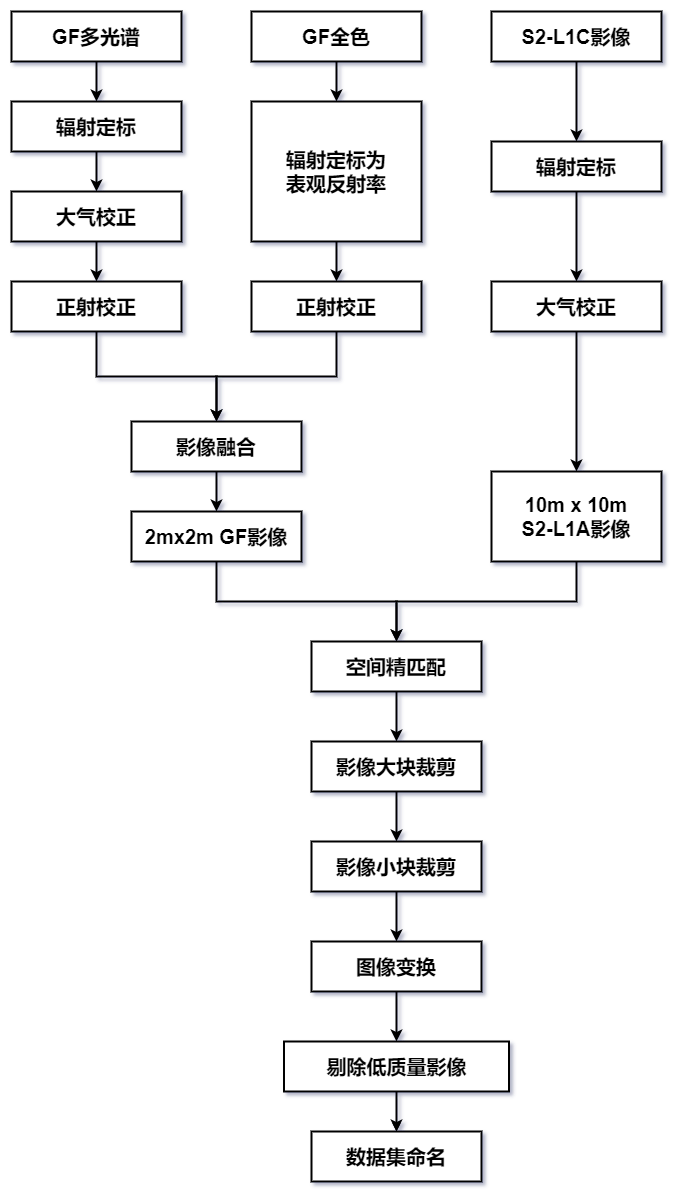
\includegraphics[height=6cm]{pic/chap0201.png}
            \caption{数据集制作流程}
            \label{fig:0201}
        \end{figure}

        \column{0.6\textwidth}
        \begin{enumerate}
            \item 高分影像预处理, 数据融合
            \item 哨兵影像预处理
            \item 大块裁剪的哨兵影像与高分影像空间精匹配
            \item ROI设置, 大块影像对裁剪
            \item 脚本批量小块裁剪, 哨兵400, 高分2000
            \item 影像对色彩匹配
            \item 剔除少量含云雾影像
            \item 数据集重命名
        \end{enumerate}
    \end{columns}
    
\end{frame}

\subsection{ESRGAN结果}

\begin{frame}{当前章节}
    \tableofcontents[currentsection, currentsubsection]
\end{frame}

\begin{frame}{定性分析}
    \begin{figure}
        \centering
        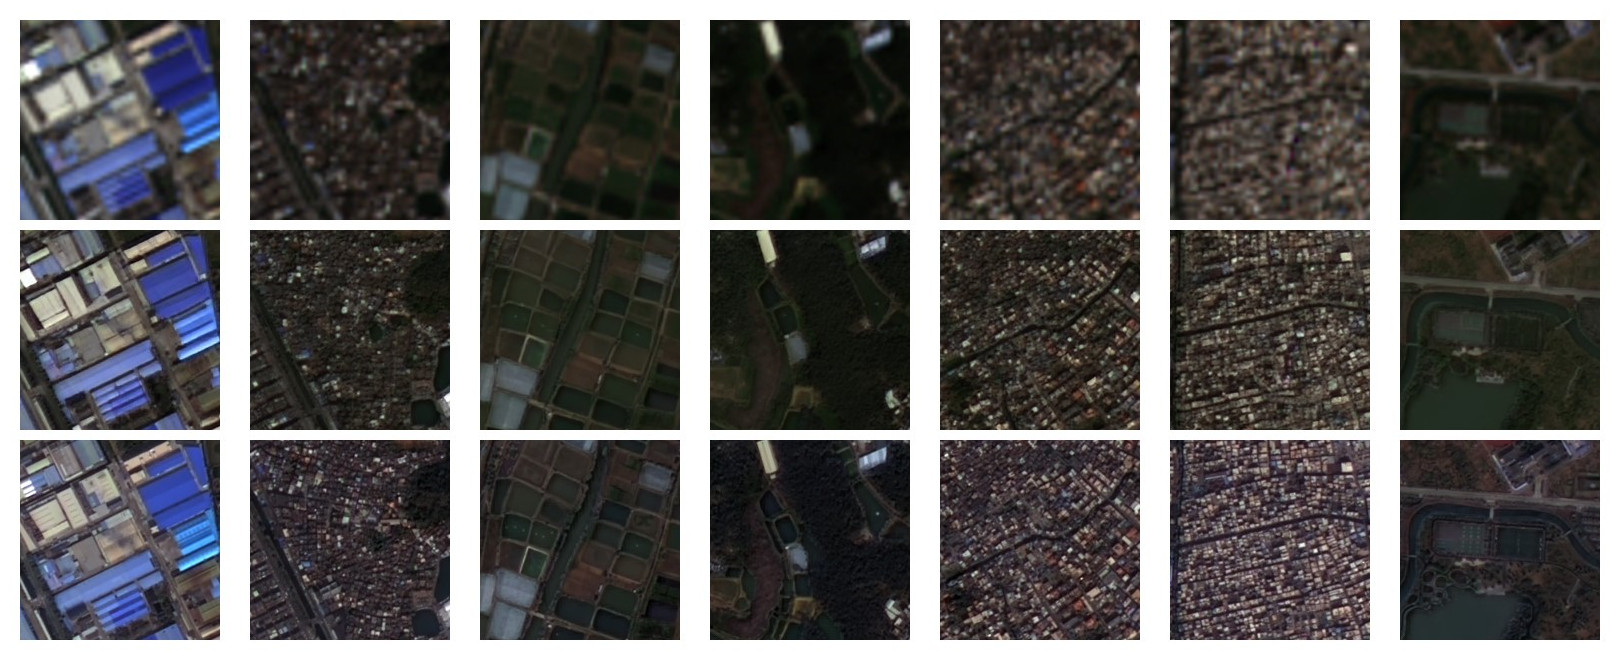
\includegraphics[width=\textwidth]{pic/chap0202.jpg}
        \caption{ESRGAN结果\\从上至下依次为Bicubic, ESRGAN, GroudTruth}
        \label{fig:0202}
    \end{figure}
\end{frame}

\begin{frame}{定量分析}
    \begin{table}[h]
        \centering
        \begin{tabular}{ m{3cm} | m{3cm} | m{3cm}  }
            \hline
            \scriptsize{SSIM/PNSR} & \scriptsize{Bicubic} & \scriptsize{ESRGAN} \\ \hline       
            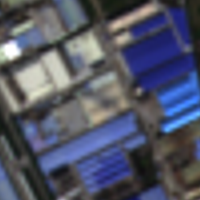
\includegraphics[height=0.7cm]{pic/chap020301.png} \scriptsize{厂房}
            & \scriptsize{0.33/17.06}
            & \scriptsize{0.72/21.95} \\ 
            \hline
            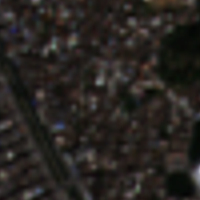
\includegraphics[height=0.7cm]{pic/chap020302.png} \scriptsize{居民楼}
            & \scriptsize{0.27/19.60}
            & \scriptsize{0.52/22.99} \\
            \hline
            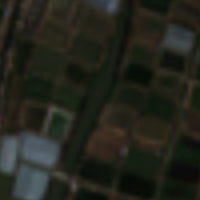
\includegraphics[height=0.7cm]{pic/chap020303.png} \scriptsize{农田}
            & \scriptsize{0.57/24.25}
            & \scriptsize{0.76/28.40} \\
            \hline
            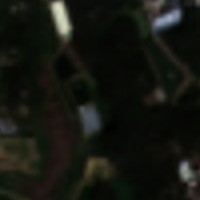
\includegraphics[height=0.7cm]{pic/chap020304.png} \scriptsize{森林}
            & \scriptsize{0.52/22.91}
            & \scriptsize{0.70/26.79} \\
            \hline
            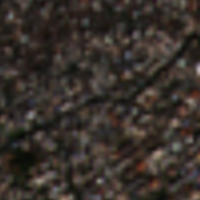
\includegraphics[height=0.7cm]{pic/chap020305.png} \scriptsize{城镇1}
            & \scriptsize{0.17/18.22}
            & \scriptsize{0.50/19.75} \\
            \hline
            
\includegraphics[height=0.7cm]{pic/chap020306.png} \scriptsize{城镇2}
            & \scriptsize{0.15/16.61}
            & \scriptsize{0.43/17.58} \\
            \hline
            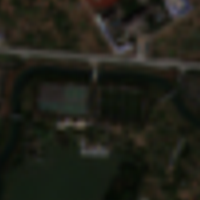
\includegraphics[height=0.7cm]{pic/chap020307.png} \scriptsize{湖水}
            & \scriptsize{0.54/23.33}
            & \scriptsize{0.67/27.24} \\
            \hline
        \end{tabular}
        
      \end{table}
    
\end{frame}

\subsection{结果分析}

\begin{frame}{当前章节}
    \tableofcontents[currentsection, currentsubsection]
\end{frame}

\begin{frame}{结果分析}
    对于结果分析:
    \begin{itemize}
        \item 深度学习超分较于传统方法提高了超分整体质量(SSIM)
        \item 深度学习超分方法在细节提升方面还有待提高(PNSR, 城镇)
    \end{itemize}
    同时也存在问题:
    \begin{itemize}
        \item 异源遥感超分影像, 训练崩溃
        \item 定性分析时, 如何排除色调差异
    \end{itemize}
    工作安排:
    \begin{itemize}
        \item 学习模型信息, 探究训练崩溃原因
        \item 探究迁移学习(finetune)对超分结果影响
    \end{itemize}
\end{frame}